
%%% Local Variables:
%%% mode: latex
%%% TeX-master: t
%%% End:

\documentclass[11pt]{article}

\usepackage{booktabs}
\usepackage{framed}
\usepackage[left=22mm,right=22mm,top=25mm,bottom=25mm]{geometry}
\usepackage{parskip}

% Figures
\usepackage{subfig}

% Maths
\usepackage{amsmath,amssymb,amsthm}

\newtheorem{theorem}{Theorem}[section]
\newtheorem{corollary}{Corollary}[theorem]
\newtheorem{lemma}[theorem]{Lemma}

% Algorithms
\usepackage[noend]{algpseudocode}
\usepackage{algorithm}

% TikZ
\usepackage{tikz}

\usetikzlibrary{arrows,topaths,calc,shapes,through,intersections}

\tikzstyle{vertex}=[circle,fill=black,minimum size=10pt,inner sep=0pt]
\tikzstyle{dual}=[draw,circle,minimum size=10pt,inner sep=0pt]
\tikzstyle{edge} = [draw,very thick,-]
\tikzstyle{weight} = [font=\small]

\newcount\mycount

% Other
\newcommand{\ra}[1]{\renewcommand{\arraystretch}{#1}}

\title{Single-Source Shortest Paths in Planar Graphs}
\author{Stuart Baker, \"{O}mer Cerraho\u{g}lu, Sebastian Claici}
\date{}

\begin{document}
\maketitle

\begin{abstract}
  We survey advances in single-source shortest paths algorithms on the special case of planar graphs. For the case of non-negative edge weights, we show $\mathcal{O}(n\log \log n)$ algorithm and provide intuition for an optimal $\mathcal{O}(n)$ algorithm. For arbitrary edge weights, we give an $\mathcal{O}(n\log^2 n)$ algorithm and show how to modify it to achieve $\mathcal{O}(n\log^2 n/\log \log n)$.
\end{abstract}

\section{Introduction}
\label{sec:introduction}

Finding shortest paths in graphs is one of the oldest combinatorial optimization problems. At least in the sense of path finding, there are references dating back to the late 1800's~\cite{wiener1873ueber}. The standard algorithm for single-source shortest paths on a graph with no negative edge weights is Dijkstra's algorithm~\cite{dijkstra1959note}.

While for general graphs the problem has been effectively solved for decades, the special case where the graph is planar has seen a number of surprising developments in recent years. We enumerate these here, and detail them in later sections.

For directed graphs where the edge weights are non-negative, the first improvement over $\mathcal{O}(n\log n)$ came from Federickson who gave a $\mathcal{O}(n \sqrt{\log n}$) bound~\cite{federickson1987fast}. This was improved nearly a decade later by Henzinger et al.\ to linear time~\cite{henzinger1997faster}. We remark that for general \emph{undirected} graphs with positive edge weights, there are known linear time algorithms for single-source shortest paths in the RAM model~\cite{thorup1999undirected}.

For directed graphs with arbitrary edge weights, recent developments greatly improve upon the naive $\mathcal{O}(n^2)$ of Bellman-Ford. In 2010, Klein, Mozes and Weimann gave a $\mathcal{O}(n \log^2 n)$ algorithm~\cite{klein2010shortest}, which was improved to $\mathcal{O}(n \log^2 n / \log \log n)$ shortly thereafter~\cite{mozes2010shortest}. Both algorithms make use of a $\mathcal{O}(n \log n)$ multiple-source shortest paths algorithm due to Klein~\cite{klein2005multiple}.

The goal of this paper is to provide intuition into some of the recent developments in planar graph theory.

This paper is organized as follows: in section~\ref{sec:background} we provide background on the theorems we will need later on; in section~\ref{sec:graph-sep} we detail planar graph separators, which are used extensively in divide-and-conquer planar graph algorithms. In sections~\ref{sec:nonn-edge-weights}~and~\ref{sec:arbitr-edge-weights} we detail faster algorithms for single-source shortest paths in graphs with non-negative, respectively negative edge weights.

\section{Background}
\label{sec:background}

We assume the reader is familiar with basic graph theory. Planar graphs are graphs that can be drawn in Euclidean space such that no two edges cross each other. Every drawing of a planar graph delineates several faces, one of which is unbounded and represents the ``outside'' of the graph; we call this face the infinite face, and denote it by $f_{\infty}$. The following theorems are used implicitly or explicitly throughout the paper.\\

\begin{theorem}[Jordan curve theorem]
  Let $C$ be any closed curve in the plane. Removal of $C$ divides the plane into exactly two connected regions, the ``inside'' and the ``outside'' of $C$.
\end{theorem}

An interesting proof of the Jordan curve theorem that uses the non-planarity of the complete bipartite graph on two sets of 3 edges ($K_{3,3}$ shown in figure~\ref{fig:kuratowski}b) was given in~\cite{thomassen1992jordan}.\\

\begin{theorem}[Euler's formula for planar graphs]
  If $n$ is the number of nodes, $m$ the number of edges, and $f$ the number of faces of a planar graph, the following formula holds:
\[
  n - m + f = 2.
\]
\end{theorem}

From Euler's formula, we can quickly prove a bound on the number of edges in a planar graph:\\

\begin{theorem}
  Any $n$-vertex planar graph with $n \geq 3$ contains no more than $3n-6$ edges.\\
\end{theorem}

\begin{theorem}[Kuratowski's theorem]
  A graph is planar if and only if it contains neither a complete graph on five vertices, nor a complete bipartite graph on two sets of three vertices as a subgraph.
\end{theorem}

An in-depth discussion of Kuratowski's theorem and a short proof are found in~\cite{thomassen1981kuratowski}. The Kuratowski subgraphs are shown in figure~\ref{fig:kuratowski}. An immediate corollary of Kuratowski's theorem is that we can shrink edges and subgraphs while preserving planarity.\\

\begin{corollary}
  Shrinking any edge of a planar graph to a single vertex preserves planarity. Applying this inductively, shrinking any subgraph to a single vertex preserves planarity.\\
\end{corollary}

\begin{figure}[!htb]
  \centering
  \subfloat[]{
    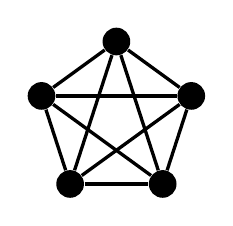
\begin{tikzpicture}[scale=0.2]
      \foreach \ang/\id in {18/1,90/2,162/3,234/4,306/5}{
        \node[vertex] (\id) at (\ang:5) {};
      }
      \foreach \number in {1,...,4}{
        \mycount=\number
        \advance\mycount by 1
        \foreach \numbera in {\the\mycount,...,5}{
          \path[edge] (\number) edge (\numbera);
        }
      }

    \end{tikzpicture}
  }\hfil
  \subfloat[]{
    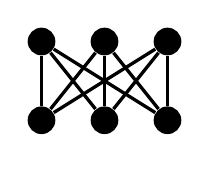
\begin{tikzpicture}[scale=0.2]
      \node at (0,-1) {};
      \foreach \x/\id in {-4/1,0/2,4/3}{
        \node[vertex] (\id) at (\x,0) {};
      }
      \foreach \x/\id in {-4/4,0/5,4/6}{
        \node[vertex] (\id) at (\x,5) {};
      }

      \foreach \x in {1,2,3}{
        \foreach \y in {4,5,6}{
          \path[edge] (\x) -- (\y);
        }
      }

    \end{tikzpicture}
  }
  \caption{Kuratowski subgraphs. (a) $K_5$, (b) $K_{3,3}$}
  \label{fig:kuratowski}
\end{figure}


\begin{theorem}
  Every planar graph can be embedded without edge crossings on a sphere. As a corollary, every node $v$ of a planar graph can be embedded on the boundary of the infinite face $f_{\infty}$.
\end{theorem}

A stereographic projection can be used to embed nodes on a plane onto a sphere without edge crossings (see figure~\ref{fig:stereo}).

\begin{figure}[!htb]
  \centering
  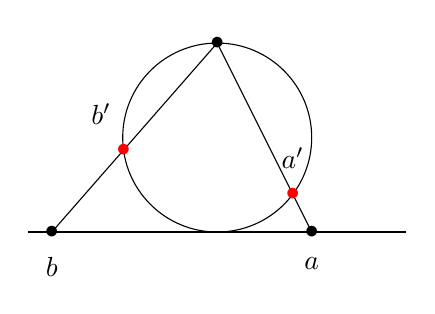
\begin{tikzpicture}[scale=0.6]
    \draw (-4,0) -- (4,0);

    \coordinate (aux) at (0,0);
    \coordinate (z) at (0,4);
    \coordinate (a) at (2,0);
    \coordinate (b) at (0,2);
    \coordinate (d) at (-3.5,0);

    \node (A) [label=270:$a$] at (a) {$\bullet$};
    \node (D) [label=270:$b$] at (d) {$\bullet$};
    \node (Z) at (z) {$\bullet$};

    \node (circ) at (b) [draw,circle through=(aux)] {};
    \coordinate (az) at (intersection 1 of circ and z--a);
    \coordinate (dz) at (intersection 1 of circ and z--d);

    \draw (a) -- (z);
    \draw (d) -- (z);

    \node (xx) [label=90:$a'$] at (az) {\color{red}$\bullet$};
    \node (yy) [label=100:$b'$] at (dz) {\color{red}$\bullet$};

  \end{tikzpicture}
  \caption{Stereographic projection of two points on a line onto a circle.}
  \label{fig:stereo}
\end{figure}

Finally, specifically for shortest paths algorithms, we note the following:\\

\begin{theorem}
  A planar graph on $n$ nodes can be transformed by adding $\mathcal{O}(n)$ nodes and edges into another planar graph such that every node has in- and out-degree at most $2$.
\end{theorem}

\section{Planar Graph Separators}
\label{sec:graph-sep}

% TODO Last point in Tarjan's algorithm
% TODO Change node to node

For large planar graphs, divide-and-conquer is a common approach to solving many kinds of problems. The core problem in divide-and-conquer problems is finding a way to divide the problem space into smaller spaces and recurse until we reach a subspace that is small enough to allow for effective computation. The base case is when the recursion reaches a subspace that contains fewer than some set number of nodes. The results at the lowest level are then rolled back up through the recursion to give the final answer. The key challenge is finding a way to divide the data set for processing.

In planar graphs, one method of dividing the graph into distinct regions is to remove a small set of nodes that bridge together the regions. By removing a small group of nodes, referred to as the separator, the nodes can be broken into two disjoint sets. The goal of finding the separator is to minimize the number of nodes required to separate the graph.

\subsection{Fundamental Cycle Separators}
\label{sec:graph-sep-fund-cycle-sep}

Many methods for finding separators in planar graphs take a two-step approach. First, find a way of reducing the diameter of the graph. Second, search within the reduced diameter graph for a separator. One method for dividing a planar graph into smaller set was developed by Lipton and Tarjan called the fundamental cycle separator~\cite{lipton1979separator}. Lipton and Tarjan showed the following lemma: \\

\begin{lemma}
    \label{lemma:separator}
    for any planar graph $G = (V,E)$ on $n = |V|$ nodes, and for any weight function $w: V \rightarrow \mathbb{R}^+$, it is possible to partition the nodes of the graph into three sections $A, B$ and $S$ such that
    \begin{itemize}
        \item $w(A), w(B) \leq \alpha \cdot w(V)$ for some $\alpha \in (0,1)$
        
        \item There are no edges between nodes in $A$ and nodes in $B$.
        
        \item The size of the separator $S$ is small. In particular, we can achieve $|S| = \mathcal{O}(\sqrt{n})$.
    \end{itemize}
\end{lemma}

For a root node $r$, we can build a spanning tree of the graph $G$ that has depth $d$. We define $T^*$ as the dual tree of the triangulated version of $G$. To triangulate a graph, we add extra edges to the graph such that every face of the graph has no more than three edges. Taking the dual of the tree means to create a new graph that has a node for each face in the original graph, and an edge between any two faces that shared a boundary. From this tree, every non-tree edge $e$ defines a fundamental cycle $C(e)$. A fundamental cycle is a distinct cycle created when you add any non-tree edge from a graph to that graph's spanning tree. Since the depth of $T$ is at most $d$, we know that $|C(e)| \leq 2d + 1$. However, because the diameter of $G$ may be large, we want to reduce it so that we can constrain $|C(e)| \leq \sqrt{n}$. Central to developing this better partition is the ability to divide the planar graph into levels.

Using a weight function allows for greater generality and applicability of the algorithm. Specifically, applying the weight evenly across the nodes is particularly useful. By giving each node a weight of $\frac{1}{n}$, $A$ will have at most $\frac{2}{3}$ of the nodes, $B$ will have at most $\frac{1}{3}$ of the nodes, and the separator will be at most $\sqrt{n}$ nodes.

Given some $n$-node planar graph $G$ with nonnegative node costs, it is possible to partition the nodes of the graph based on their distance from a node $v$. One way of defining this distance is the distance from $v$ in a breadth-first search from $v$. Given the partitioning, define $L(l)$ as the number of nodes on the level $l$. The levels range from $0$ to $r$ where $r$ is the maximum distance from $v$ to any node in the graph. For the algorithm to work, an additional empty level must be added at $r+1$.

The algorithm is as follows:
\begin{enumerate}
    
    \item Find the most costly (highest weight) component in the graph and run a depth-first search from this graph. This calculates the level of each node in the graph. Find the maximum depth $r$ in the level tree, and add an additional level at $r+1$ that contains no nodes. This step can be performed in $\mathcal{O}(n)$.
    
    \item Find the level $i_0$ that contains the median node. This is the level where
    \[
    \sum_{i \leq i_0} |L_i(v)| \geq \frac{n}{2} \quad \text{and}\quad \sum_{i \geq i_0} |L_i(v)| \geq \frac{n}{2}.
    \]
    This step can be performed in $\mathcal{O}(n)$.n
    
    \item Find levels $i_- \leq i_0 \leq i_+$ such that the number of nodes on levels $i_-$ and $i_+$ is less than $\sqrt{n}$. Note that any level
    \begin{itemize}
        \item Start from the median node containing level $i_0$ and increase $i_+$ as well as decrease $i_-$ until $|L_{i_-}|,|L_{i_+}| \leq \sqrt{n}$
        
        \item Because each section can only contain half of the nodes, we can use the counting argument to state that $|i_0 - i_-|,|i_+ - i_0| \leq \frac{\sqrt{n}}{2}$
        
        \item This gives a separator $|L_{i_-} \cup L_{i_+}| \leq 2 \sqrt{n}$, which we can return if the grouping of $L_{< i_-}$, $L_{> i_+}$, and $L_{i_-,i_+}$ is balanced.
    \end{itemize}
    If the grouping is not balanced, continue to step $4$.
    
    \item Form a condensed graph $G^{'}$ by deleting  all edges in $L_{\geq i_+}$, and contracting all edges in $L_{\leq i_-}$ into a super node $v$ that is connected to all nodes in $L_{i_- + 1}$.
    
    \item From the condensed graph $G^{'}$, create a fundamental cycle separator $C$
    \begin{itemize}
        \item Build a breadth-first tree from $v$. This tree will have depth $|i_+ - i_-| \leq \sqrt{n}$
        
        \item Add edges to the tree such that each face (except $f_{\infty}$) is a triangle.
    \end{itemize}
    
    \item Start with any non-tree edge $uv$, and walk along the BFS tree in both directions until a cycle is formed. This cycle is the current separator candidate. Determine which side of the cycle has greater weight and call it the ``inside''.
    
    \item If the weight of the ``inside'' is larger than $2/3$, fix the cycle by changing $uv$ with another non-tree edge. We can ensure that the weight of the ``inside'' will only decrease during this process. Repeat this step until a suitable cycle separator has been found.
    
    \item Using this separator, return $A$ and $B$ as some combination of interior$(C)$, exterior$(C)$, $L_{< i_-}$, and $L_{> i_+}$. $S$ can be returned as a combination of $L_{i_-}$, $L_{i_+}$, and $C$.
    
\end{enumerate}

\subsection{Miller's Algorithm}
\label{sec:graph-sep-miller}

Miller showed an alternative method for separating a planar graph into two sections with a separator region. He showed that every 2-connected, triangulated planar graph with $n$ nodes has a simple cycle $C$ of length at most $4\sqrt{n}$~\cite{miller1984finding}. Like Lipton and Tarjan's algorithm, Miller's algorithm works to reduce the diameter of the graph and then find the separator within the reduced-diameter graph. The key difference the methods is the way in which Miller reduces the diameter. Instead of looking for the median node, Miller searches for the heaviest subtree in the BFS tree. This is found by following the heaviest child until you reach a cycle $C_0$ with weight $> \frac{1}{2}$, but where all enclosed cycles have weight $< \frac{1}{2}$. From there, Miller finds the limits on the region by searching for the level $i_-$ higher in the BFS tree that has a boundary size of $\mathcal{O}(\sqrt{n})$, and the level $i_+$ lower in the BFS tree than $i_0$ that has  a boundary size of less than $\mathcal{O}(\sqrt{n})$.

\subsection{r-Subdivision}
\label{sec:graph-sep-rsub}

A division into $2$ regions is not useful for a divide-and-conquer approach, but the concept can be expanded further to develop a useful approach. Fortunately, we can achieve an $r$-segmentation of the graph into $\Theta \left (\frac{n}{r} \right )$ regions, each with $\mathcal{O}(r)$ nodes, and separated by $\mathcal{O} \left (\frac{n}{\sqrt{r}} \right )$ boundary nodes. The boundary nodes are those nodes that are connected to more than one subgraph. Federickson takes this definition a step further and defines a \textit{suitable} r-division of a planar graph as the r-division that satisfies two characteristics~\cite{federickson1987fast}:
\begin{enumerate}
    \item Each boundary node is contained in at most three regions
    
    \item Any region that is not connected consists of connected components, all of which share boundary nodes with exactly the same set of either one or two connected regions.
\end{enumerate}
A suitable $r$-division is shown in figure~\ref{fig:rsep}.

\begin{figure}[!htb]
    \centering
    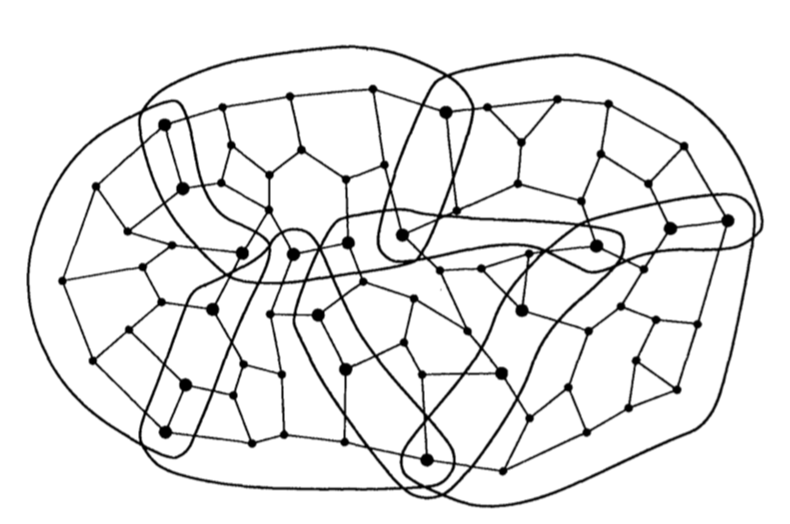
\includegraphics[width=.5\textwidth]{rsep}
    \caption{Planar graph separated into $r$ regions. From~\cite{federickson1987fast}.}
    \label{fig:rsep}
\end{figure}

Starting with the initial graph $G$, all of the nodes are in the interior region. A separator algorithm can then be applied to the graph with all of the node weights set to $\frac{1}{n}$. This will produce three sets: $A$, $B$, and $C$. From these two sets, we can infer two regions that have the node sets $A_1 \subseteq A \cup C$ and $A_2 \subseteq B \cup C$. These two node sets will have sizes $\alpha n + \mathcal{O}\sqrt{n}$ and $(1 - \alpha) n + \mathcal{O}\sqrt{n}$ with $\frac{1}{3} \leq \alpha \leq \frac{2}{3}$. To continue the process, the separator algorithm can be recursively applied to any region that has more than $r$ nodes. The total runtime of this algorithm is $\mathcal{O} \left (n \log \left (\frac{n}{r} \right ) \right )$. This process can be performed significantly faster, as demonstrated by Henzinger, to create $r$-division in $\mathcal{O}(n)$ time~\cite{henzinger1997faster}.

\section{Single source shortest paths with non-negative edge weights}
\label{sec:nonn-edge-weights}

The fastest algorithm for single-source shortest paths in general graphs with non-negative edge weights is Dijkstra's algorithm which runs in time $\mathcal{O}(m + n\log n)$. Planar graphs are sparse, so simply applying Dijkstra's algorithm on a planar graph already yields an $\mathcal{O}(n \log n)$ algorithm.

We can do much better by using the ideas developed in section~\ref{sec:graph-sep}.

\subsection{Simple algorithm}
\label{sec:simple-algorithm}

A simple $\mathcal{O}(n\sqrt{\log n \log \log n})$ emerges beautifully from an $r$-division if we set $r = \log n/\log \log n$. The first step is to compute the single-source shortest paths for each boundary node in each region $R$. As customary, we use $s$ for the source node throughout this section.


\begin{algorithm}[!htb]
  \refstepcounter{algorithm}
  \label{alg:sssp-region}
  \begin{algorithmic}
    \ForAll {Regions $R$}
      \ForAll {Boundary nodes $v \in R$}
        \State Compute SSSP from $v$ in $R$
        \State Store $(u,v)$ distances for any two boundary nodes $u$, $v$
      \EndFor
    \EndFor
  \end{algorithmic}
\end{algorithm}

 We can now replace each region $R$ by a complete graph on $R$'s boundary nodes with shortest paths distances between any two nodes. Call this auxiliary graph $G'$. The second phase of the algorithm is to compute the SSSP from $s$ in $G'$. This gives the true shortest paths from $s$ to all the boundary nodes. Finally, we must tidy up by finding the distances from $s$ to the nodes inside each region.

\begin{algorithm}[!htb]
  \refstepcounter{algorithm}
  \label{alg:sssp-full}
  \begin{algorithmic}
    \ForAll {Regions $R$}
      \ForAll {Boundary nodes $v \in R$}
        \State Set $d(v) = d_{G'}(s,v)$
        \State Compute SSSP from $v$ in $R$
      \EndFor
    \EndFor
  \end{algorithmic}
\end{algorithm}

To analyze the algorithm, recall the properties of an $r$-division.
\begin{itemize}
\item Total number of boundary nodes is $\mathcal{O}(n/\sqrt{r})$.
\item Number of nodes in $G'$ is $\mathcal{O}(n/r)O(\sqrt{r})=O(n/\sqrt{r})$.
\item Number of edges in $G'$ is $\mathcal{O}(n/r)\mathcal{O}(r) = \mathcal{O}(n)$.
\end{itemize}

Using $r=\frac{\log n}{\log \log n}$, the first phase is bounded above by
\[
  O\left(n\frac{\sqrt{\log \log n}}{\sqrt{\log n}} \log n\right)= O(n \sqrt{\log n \log \log n}),
\]
the second phase is an SSSP in a size $\mathcal{O}(n \frac{\sqrt{\log \log n}}{\sqrt{\log n}})$ graph, and thus also $\mathcal{O}(n \sqrt{\log n \log \log n})$, while the tidying up is a series of SSSPs in each of the regions, and has the same bound as the first phase---$\mathcal{O}(n \sqrt{\log n \log \log n})$. The total time bound ends up $\mathcal{O}(n \sqrt{\log n \log \log n})$.

\subsection{Recursive subdivisions}
\label{sec:recursion}

We have improved upon Dijkstra's algorithm, but there is still room to do better. A recursive subdivision $\bar{r} = (r_0, \ldots, r_h)$ of a graph is a division in which the regions are subdivided recursively up to edges. A region at level $i$ is sub-divided into regions of size $r_{i-1}$. The regions at level $0$ are called atomic and contain only one edge $uv$.

For each region $R$, we maintain a priority queue $Q(R)$ that stores the subregions of $R$ if $R$ is nonatomic, or the single arc $uv$ is $R$ is atomic. We call and edge $uv$ \emph{active} if its head $v$ has a finite distance label $d(v)$, and \emph{inactive} if $d(v)$ is infinite. During execution, edges can change status from \emph{active} to \emph{inactive} several times. The algorithm ensures that for every region $R$, the minimum element of $Q(R)$ is the minimum label $d(v)$ over all edges $vw$ in $R$ that remain to be processed.

We would like to apply Dijkstra's until completion in each region, and somehow bubble up the results on lower levels. Unfortunately, this idea does not lead to a faster algorithm. Instead, we try to work mostly on the lower levels and perform speculative work. The algorithm tries to ensure that, on average, the operations on large queues can be paid for by the many operations performed on small queues.

\begin{algorithm}
  \refstepcounter{algorithm}
  \label{alg:linear}
  \begin{algorithmic}[1]
    \State Find recursive subdivision $R(G), R(P_i), \ldots, R(uv)$
    \State Allocate queue $Q$ for each region
    \State $d(v) \gets \infty, \forall v$
    \State $d(s) \gets 0$
    \ForAll {$sv \in E(G)$}
      \State \Call{Update}{$R(sv),sv,0$}
    \EndFor
    \While {$Q(R(G)).minKey() < \infty$}
      \State \Call{Process}{$R(G)$}
    \EndWhile
  \end{algorithmic}
\end{algorithm}

Each call to \textsc{Process} is effectively an invocation of Dijkstra's algorithm. If we're at the level of an edge, we try to relax that edge. Otherwise, we recursively call \textsc{Process} on the current best subregion to explore further.

\begin{algorithm}[!h]
  \label{alg:process}
  \begin{algorithmic}[1]
    \Procedure{Process}{}
      \If {$R$ contains only $uv$}
        \If {$d(v) > d(u) + c(u,v)$}
          \State $d(v) \gets d(u) + c(u,v)$
          \State for each outgoing edge $vw$ of $v$, call \Call{Update}{$R(vw),vw,d(v)$}
        \EndIf
        \State $Q(R).updateKey(uv,\infty)$
      \Else
        \Repeat
          \State $R' \gets Q(R).getMin()$
          \State \Call{Process}($R'$)
          \State $Q(R).updateKey(R',Q(R').minKey())$
        \Until {$Q(R).minKey()$ is infinity or if repeated $\alpha_{h(R)}$ times}
      \EndIf
    \EndProcedure
  \end{algorithmic}
\end{algorithm}

The calls to \textsc{Update} ensure that the information in parent regions stays consistent with work done at lower regions by bubbling up key updates that result in a new minimum.

\begin{algorithm}[!h]
  \label{alg:update}
  \begin{algorithmic}[1]
    \Procedure{Update}{$R,x,k$}
      \State $Q(R).updateKey(x,k)$
      \If {$updateKey$ reduced the value of $Q(R).minKey()$}
        \State \Call{Update}{$parent(R),R,k$}
      \EndIf
    \EndProcedure
  \end{algorithmic}
\end{algorithm}

Unlike Dijkstra's algorithm, the work we do in a region is only speculative. Often we cannot afford to fully process a region, and executions are stopped after a fixed number of steps. Specifically, at level $i$, we perform $\alpha_i$ steps of Dijkstra's algorithm, where the $\alpha_i$ are parameters that will dictate the running time of the algorithm.

\subsubsection{Correctness}
\label{sec:correctness}

Recall from Dijkstra's algorithm that three properties imply correctness:
\begin{enumerate}
\item Initialization: $d(s) = 0$.
\item Minimum length property: $d(v)$ is an upper bound on the $s$ to $v$ distance
\item All edges are relaxed. We call an edge $uv$ is relaxed if $d(v) \leq d(u) + c(u,v)$.
\end{enumerate}

The first property is true at the start of the algorithm, and remains true throughout. The following lemma establishes the second property:\\

\begin{lemma}
  For each node $v$, $d(v)$ is an upper bound on the distance from $s$ to $v$ throughout the algorithm.
\end{lemma}

\begin{proof}
  Initially, all labels except $d(s)$ are infinity. The labels only get changed in line $4$ of \textsc{Process}, and assuming inductively that the old labels $d(v)$ and $d(u)$ are upper bounds on the distance to $u$ and $v$, it follows that the new labels will also be upper bounds.
\end{proof}

The following three lemmas establish the third property.\\

\begin{lemma}
  If an edge $uv$ is inactive then it is relaxed.
\end{lemma}

\begin{proof}
  The lemma holds before the first call to \textsc{Process} as every node but $s$ has label infinity and outgoing edges from $s$ are active. Edges are deactivated only in line $7$ of \textsc{Process} which occurs only after the edge has been relaxed.

  Note that it is possible that an edge becomes unrelaxed after changes to the labels of its endpoints. This can occur for a call to \textsc{Update}, but line $2$ of \textsc{Update} changes the key of the edge, making it active again.
\end{proof}

\begin{lemma}
  The key of an active edge $uv$ is $d(u)$ (except during lines $3-6$ of \textsc{Process}).
\end{lemma}

\begin{proof}
  Whenever a label $d(u)$ is assigned a value $k$, \textsc{Update}$(R(uv),uv,k)$ is called for each outgoing edge $uv$, and the key of $uv$ is updated to $k$.
\end{proof}

\begin{lemma}
  \label{lemma:invariant}
  For any region $R$ that is not an ancestor of the current region, the key associated with $R$ in $Q(parent(R))$ is the minimum key of $Q(R)$.
\end{lemma}

\begin{proof}
  Whenever the minimum key of a queue $Q(R)$ is changed in line $2$ of \textsc{Update}, the recursive call in line $4$ ensures that the key associated with $R$ in the parent of $R$ is also changed.
\end{proof}

From lemma~\ref{lemma:invariant}, the following corollary follows:\\

\begin{corollary}
\label{cor:relaxed}
  For any region $R$ that is not an ancestor of the current region,

  \[
    Q(R).\text{minKey}() = \min \{ d(v) | \text{uv is a pending edge contained in R} \}
  \]
\end{corollary}

When the algorithm terminates, the minimum key of the priority queue associated with the entire graph will be infinity, and by corollary~\ref{cor:relaxed} all edges will be relaxed.

\subsubsection{Analysis}
\label{sec:analysis}

We show that dividing the graph into $\mathcal{O}(n/\log^4n)$ regions of size $\mathcal{O}(\log^4 n)$ with boundaries of size $\mathcal{O}(\log^2 n)$ and setting $\alpha_0 = 0, \alpha_1 = \log n$ and $\alpha_2 = 1$ yields an $\mathcal{O}(n \log \log n)$ single source shortest paths algorithm. The $\alpha_i$ are parameters that dictate how much speculative work we do in a region before moving on. Note that this division is simply an $r$-division with $r=\log^4 n$, and thus $r_0=1, r_1 = \log^4 n$, and $r_2 = n$.

We restate the algorithm:
\begin{enumerate}
\item Select the region containing the lowest labeled node that has active outgoing edges in the region.
\item Repeat $\log n$ times: Select the lowest labeled node $v$ in the current region that has active outgoing edges in the region. Relax and deactive its outgoing edges $vw$ in that region. For each of the other endpoints $w$ of these edges, if relaxing the edge $vw$ resulted in decreasing the label of $w$, then activate the outgoing edges of $w$.
\end{enumerate}

The majority of the time is spent in invocations of \textsc{Process}. We say that an invocation of \textsc{Process} on region $R$ is \emph{truncated} if $Q(R).minKey()$ is infinity at the end of the invocation. All level $0$ invocations are truncated. The crux of the analysis relies on the following \emph{charging invariant}:

\noindent\makebox[\textwidth][c]{%
\begin{minipage}{.8\textwidth}
  For any pair $(R,v)$ of region $R$ and entry node $v$, there is an invocation $B$ of \textsc{Process} such that all invocations charging to $(R,v)$ are descendants of $B$ (or $B$ itself).
\end{minipage}}

Intuitively, the \emph{charging invariant} says that the number of charges to any pair is small, so the number of truncated invocations will be small.

 Let us first consider the number of pairs $(R,v)$ on each level to which we can charge truncated invocations to (recall that $v$ is an entry node into $R$):
\begin{itemize}
\item If $R$ has level $0$, then $R$ is charged by at most one level $0$ invocation. There are $\mathcal{O}(n)$ pairs $(R,v)$ on level $0$, and thus $\mathcal{O}(n)$ chargers.
\item If $R$ has level $1$, the pair is charged by at most one level $1$ invocation and at most $\alpha_1 = \log n$ level $0$ invocations. There are $\mathcal{O}(n/\log^4n)\cdot O(\log^2 n)$ pairs on level $1$.
\item If $R$ has level $2$, then the pair is charged by at most one level $2$ invocation, at most $\alpha_2 = 1$ level $1$ invocations, and at most $\alpha_2\alpha_1 = \log n$ level $0$ invocations. There is only one pair $(R,v)$ on level $2$, namely $(R_G,s)$.
\end{itemize}

Let $s_i$ be the total number of invocations at level $i$ (truncated and non-truncated), and $t_i$ be the number of truncated chargers at level $i$.

All level $0$ invocations are truncated, thus
\[
s_0 = \mathcal{O}(n)
\]
 Each non-truncated level $j$ invocation results in $\alpha_j$ invocations at level $j-1$. Hence the number of level $1$ invocations is
\[
s_1 \leq s_0/\alpha_1 + t_1 = \mathcal{O}(n/\log n) + \mathcal{O}(n/\log^2 n).
\]
 Similarly, the total number of level $2$ invocations is
\[
s_2 \leq s_1/\alpha_2 + 1 = s_1 + 1 = \mathcal{O}(n/\log n).
\]

Let's look at the time spent per invocation at each level. We bound the time required per queue operation; since at level $i$ there are $\alpha_i$ calls to lower levels, and thus $\alpha_i$ queue operations, this gives us a time bound per invocation.

\begin{itemize}
\item At level $0$, there is only one item in the queue, so operations take constant time, and there are $\alpha_0 = 0$ calls to lower levels.
\item At level $1$, queues are of size $\mathcal{O}(log^4 n)$, so queue operations take $\mathcal{O}(\log \log n)$ time. There are $\alpha_1 = \log n$ calls to lower levels, for a total of $\mathcal{O}(\log n \log \log n)$.
\item At level $2$, queues are of size $\mathcal{O}(n/\log^4 n)$, so queue operations take $\mathcal{O}(\log n)$ time, and there are $\alpha_2 = 1$ calls to lower levels, for a total of $\mathcal{O}(\log n)$.
\end{itemize}

To get our total time bounds, we multiply the time per invocation with the number of invocations at each level, and add everything up.
\begin{align*}
  \text{Total} &= \mathcal{O}(\log n) \cdot \mathcal{O}(n/\log n) + \mathcal{O}(\log n \log \log n) \cdot \mathcal{O}(n/ \log n) + \mathcal{O}(1) \cdot \mathcal{O}(n) \\
               &= \mathcal{O}(n \log \log n)
\end{align*}
The information is summarized in table~\ref{tab:process}.


\begin{table*}[!h]\centering
\caption{Time required for \textsc{Process} calls.}
\label{tab:process}
\ra{1.3}
\begin{tabular}{@{}llllll@{}} \toprule
  Level & Calls & Time per invocation & No.\ $(R,v)$ pairs & No.\ invocations & Total time\\ \midrule
  $2$ & $1$ & $\mathcal{O}(\log n)$ & 1 & $\mathcal{O}(n/\log n)$ & $\mathcal{O}(n)$\\
  $1$ & $\log n$ & $\mathcal{O}(\log n \log \log n)$ & $\mathcal{O}(n/\log^2 n)$ & $\mathcal{O}(n/\log n)$ & $\mathcal{O}(n\log \log n)$\\
  $0$ & $0$ & $\mathcal{O}(1)$ & $\mathcal{O}(n)$ & $\mathcal{O}(n)$ & $\mathcal{O}(n)$\\ \midrule
  Total & & & & & $\mathcal{O}(n\log \log n)$\\
  \bottomrule
\end{tabular}
\end{table*}

The analysis bounds invocations of \textsc{Process}, but not those of \textsc{Update}. However, the analysis for \textsc{Update} follows the same direction and also yields a $\mathcal{O}(n \log \log n)$ time bound.

\subsubsection{Linear time}
\label{sec:linear-time}

To improve the running time to linear, we must use a recursive subdivision. Let $r_i$ be the size of the subregions on level $i$, and $\alpha_i$ be the number of iterations per invocation of \textsc{Process} for level $i$. Define
\[
  \alpha_i = \frac{4\log r_{i+1}}{3 \log r_i}
\]
with $\alpha_0 = 0$, and $\alpha_{h(G)} = 1$.

To achieve linear time, we define the $r_i$ inductively by $r_0 = 1$, and $r_{i+1} = 16^{r_i^{1/6}}$. This defines a division into roughly $\log^{*} n$ levels. The algorithm is given above, but we repeat it here for clarity:

\begin{algorithm}
  \begin{algorithmic}[1]
    \State Find recursive subdivision $R(G), R(P_i), \ldots, R(uv)$
    \State Allocate queue $Q$ for each region
    \State $d(v) \gets \infty, \forall v$
    \State $d(s) \gets 0$
    \ForAll {$sv \in E(G)$}
      \State \Call{Update}{$R(sv),sv,0$}
    \EndFor
    \While {$Q(R(G)).minKey() < \infty$}
      \State \Call{Process}{$R(G)$}
    \EndWhile
  \end{algorithmic}
\end{algorithm}


The correctness proof did not rely on the $\alpha_i$ or $r_i$ and follows from section~\ref{sec:correctness}. Using a very similar argument as in section~\ref{sec:analysis}, it is possible to show that the linear time bound holds for this choice of parameters, though the recursion is more involved.

\section{Single source shortest paths with negative edge weights}
\label{sec:arbitr-edge-weights}

If we exploit the sparsity of planar graphs, the running time of Bellman-Ford is $\mathcal{O}(n^2)$. We have had success so far with planar graph separators, so it should come as no surprise that using separators here also leads to large speed-ups.

In this section we assume that the source node $s$ is on the boundary of the infinite face $f_{\infty}$. Recall from section~\ref{sec:background} that we can always place a vertex on the boundary of $f_{\infty}$. We also make use of Klein's multiple-source shortest paths algorithm~\cite{klein2005multiple}. Klein's algorithm yields shortest paths from all nodes on the boundary of $f_{\infty}$ (the multiple sources) to all other nodes in $\mathcal{O}(n \log n)$ time.

\subsection{An $\mathcal{O}(n \log^2 n)$ solution}
\label{sec:first-solution}

We first provide intuition into the algorithm. As with the simple non-negative shortest paths algorithm, we first find shortest paths from boundary vertices to other boundary vertices within all subregions. We can ``glue'' shortest paths within regions together to find true shortest paths between boundary vertices of separate regions. We then tidy up by finding shortest paths within each region.

We focus on the $\mathcal{O}(n\log^2 n)$  algorithm, and provide intuition into how to modify the algorithm to achieve an $O(\log \log n)$ speed-up.

We give the high-level stages of the algorithm first. Assume that we are given a cycle separator of size $\mathcal{O}(\sqrt{n})$ that splits the graph into an outside $G_0$ and an inside $G_1$. Let $r$ be any vertex on the separator.

\begin{enumerate}

\item \textbf{Recursive call:} Recursively compute the distances from $r$ within $G_0$ and $G_1$.

\item \textbf{Intra-part boundary distances:} Use the multiple-source shortest paths algorithm of Klein to compute all distances in $G_0$ and $G_1$ between boundary vertices. Let $\delta_i(u,v)$ be the computed shortest distance between boundary vertices $u$ and $v$ in $G_i$.

\item \textbf{Single-source inter-part boundary distances:} Use $\delta_0$ and $\delta_1$ to compute a table $B$ such that $B[v]$ is the $r$-to-$v$ distance in $G$.

\item \textbf{Single-source inter-part distances:} For each $G_i$, use $d_i$ and $B$ in a Dijsktra computation to find distances in $G$ from $r$ to all vertices of $G_i$. Let $d'_i[v]$ be the $r$-to-$v$ distance in $G$.

\item \textbf{Rerooting single-source distances:} We now have distances in $G$ from $r$. Use these distances as a feasible price function to compute, using Dijkstra's, the distances from $s$ in $G$.

\end{enumerate}

The recursive steps stop when the size of $G$ is at most $2$ at which point the problem is trivial. We go into more detail on stages 2 through 4.

\subsubsection{Intra-part boundary distances}
\label{sec: intra-part boundary distances}

Pseudocode for the algorithm follows.

\begin{algorithm}[!htb]
    \refstepcounter{algorithm}
    \label{alg:region}
    \begin{algorithmic}
        \ForAll {Regions $R$}
            \State Compute a price function using the distance function from the recursive call
            \ForAll {holes $H\in R$}
                \State Make $H$ outer face, using a stereographic projection
                \State Apply Klein's algorithm with $H$ as outer face
                \State Compute distances from all vertices of $H$ to all boundary vertices of $R$
            \EndFor
        \EndFor
    \end{algorithmic}
\end{algorithm}

From the recursive call, we already have shortest path distances in each region. We can define a price function to make the edge costs non-negative, and use Klein's algorithm to compute shortest-path trees for each node on the outer face. Note that a hole here is simply a cycle separator that splits the graph into an outside and an inside. For the case where we have two regions and a $\mathcal{O}(\sqrt{n})$ separator, we can compute distances in $\mathcal{O}(n\log n)$ time. 

This procedure is illustrated in figure~\ref{fig:long-path-a}.

\subsubsection{Single-source inter-part boundary distances}

We now want to compute the distance in $G$ between any two boundary nodes. We will need the following lemma:\\

\begin{lemma}
If $v$ and $u$ are two boundary nodes, and $P$ be a simple path between them, then $P$ can be decomposed as $P=P_1P_2\ldots P_k$, where each $P_i$ is a path between two boundary nodes and is included in $G_{i \text{ mod } 2}$.
\end{lemma}

\begin{proof}
Starting at $v$, follow path $P$ until the first point not in $G_1$ is reached. Let $P_1$ be the path until that point (not including it). The point where $P_1$ ended is a boundary node, as it is in $G_1$ and $i$ has a neighbor in $G_0$. Continue this procedure until we have traversed all of $P$.
\end{proof}

This is illustrated in figure~\ref{fig:long-path-b}.

\begin{figure}[!htb]
  \centering
  \subfloat[]{
    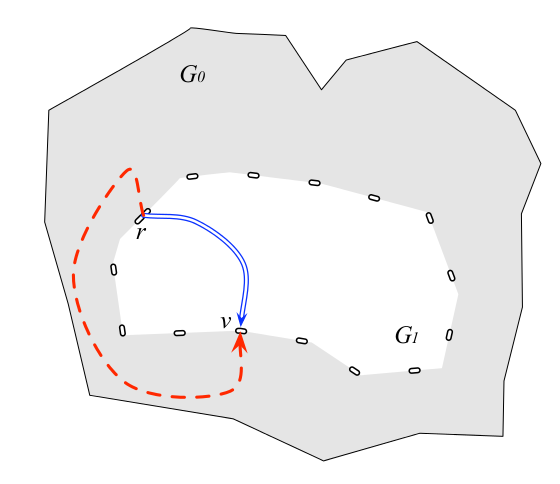
\includegraphics[width=.4\textwidth]{sssp-negative-one}
    \label{fig:long-path-a}
  }\hfil
  \subfloat[]{
    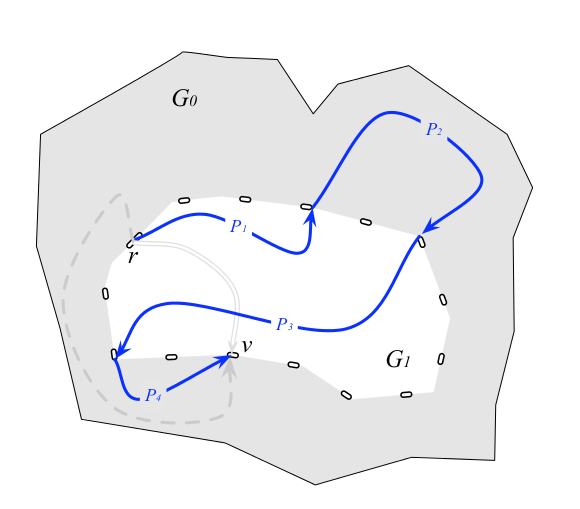
\includegraphics[width=.4\textwidth]{sssp-negative-two}
    \label{fig:long-path-b}
  }
  \caption{Path between two boundaries snakes between $G_0$ and $G_1$.}
  \label{fig:long-path}
\end{figure}

Let $V_c$ be the boundary vertices. As they form a cycle we can order the vertices in $V_c$ in trigonometric order. The algorithm is as follows:

\begin{algorithm}[!htb]
  \refstepcounter{algorithm}
  \label{alg: bellman-ford}
  \begin{algorithmic}
    \State $e_0[v] = \infty$ for all $v \in V_c$
    \State $e_0[r] = 0$
    \ForAll{ $j \ in \{1,2,\ldots,|V_c|\}$}
      \ForAll{ $v\in V_c$}
        \State $e_j[v] = \min_{w\in V_c} \{e_{j-1}[w] + \delta_i(v,w)\}$, where $i = j \mod 2$
      \EndFor
    \EndFor
    \ForAll{$v\in V_c$}
      \State $B[v] := e_{|V_c|}[v]$
    \EndFor
  \end{algorithmic}
\end{algorithm}

This algorithm resembles Bellman-Ford, with the main difference being that we have two edges for each pair of vertices. To prove correctness, we need the following lemmas:\\

\begin{lemma}
After table $e_j$ is updated, $e_j[v]$ will be the length of the shortest $r$-to-$v$ path of the form $P_1P_2\ldots P_j$, where each $P_j$ is a path in $G_{j\mod 2}$ between two boundary nodes.
\end{lemma}

\begin{proof}
We use induction. The case $j=1$ is obvious, as $\delta_i(v,w)$ is the length of the shortest $v$-to-$w$ path in $G_i$. For the induction step, suppose there were a shorter path $P' = P'_1P'_2\ldots P'_j$. Let $Q = P'_1P'_2\ldots P'_{j-1}$. Let $r$ and $u$ be the end vertices of $Q$. We know $e_j[v] \leq e_{j-1}[u] + \delta_{j\mod 2}(u,v)$. We have $\text{len}(P') = \text{len}(Q) + \delta_{j\mod 2}(u,v)$. But $e_{j-1}[u]\geq \text{len}(Q)$ (by the induction hypothesis), so $e_j[v]\leq \text{len}(P')$, thus $P'$ is not shorter than the $e_j[v]$-length path.
\end{proof}

If this algorithm were to run \textit{exactly} like Bellman-Ford, the runtime would be $|V_c|^3 = \mathcal{O}(n\sqrt{n})$, which is not the time bound we want. The improvement comes from the fact that we ordered $V_c$ trigonometrically. Specifically, note that computing $e_j[x]$ for a fixed $j$ and variable $x$ takes $|V_c|^2$ time. We will imporve this using Monge convexity as follows: let $A$ be a $|V_c|$x$|V_c|$ matrix such that $a_{kl} = e_{j-1}[v_k]+\delta_i(v_k,v_l)$. It is clear that $e_j[v_i]$ is the minima in column $j$. We will prove that the upper and lower triangles are Monge convex.\\

\begin{lemma}
For any four indices $k,k',l,l'$ such that $A_{kl}, A_{kl'}, A_{k'l}, A_{k'l'}$ are all in the upper or in the lower triangle of $A$ we have that either $$a_{kl}+a_{k'l'} \geq a_{kl'}+a_{k'l}$$ or the upper and lower triangles of $A$ are Monge convex.
\end{lemma}

\begin{proof}
Note that each term has $e_{j-1}[v_k] + e_{j-1}[v_{k'}]$ in it, so we only need to prove that $\delta_i(v_k,v_l) + \delta_i(v_{k'},v_{l'}) \geq \delta_i(v_k,v_{l'})+\delta_i(v_{k'},v_l)$. Note that $v_k,v_{k'},v_l,v_{l'}$ are cyclical in this order, and the $\delta_i$ paths all stay within one region, so the $k$-to-$l$ and $k'$-to-$l'$ paths must intersect. If $O$ is a point of intersection, the triangle inequality tells us that the sum of the $k$-to-$O$ and $O$-to-$l'$ portions of the two previous paths is at least the length of the $k$-to-$l'$ path, and similarly for the $k'$-to-$l$ path. 
\end{proof}

We can now find the column minima for both the upper and the lower triangles, and compute the minima of the two numbers per column. Using the algorithm for Monge matrices stated in section~\ref{sec:background}, we get a $|V_c|\alpha(|V_c|)$ time bound for computing all the $e_j$s, so a total time bound of $\mathcal{O}(n\alpha(n))$ where $\alpha(n)$ is the inverse Ackermann function.


\subsubsection{Single-source inter-part distances}

We want to find the distances from the fixed boundary vertex $r$ to all vertices in $G_0$ and $G_1$. Let $G_i'$ prime be the graph obtained by adding to $G_i$ a vertex $r'$ and edges between $r'$ and all boundary vertices $v$ of $G_i$ such that the length of the $(r',v)$ edge is the distance in $G$ between $r$ and $v$. Distances from $r'$ to vertices of $G_i$ are equal to distances in $G$ from $r$ to vertices of $G_i$. Let $r_{G_i}$ be the boundary vertex for which the distances in $G_i$ from $r_{G_i}$ have been computed in the recursive call. Define the following price function: $\phi(v) = d_{G_i}(r_{G_i},v)$, if $v\neq r'$ and $\phi(v) = D$ otherwise, where $D = \max_{b\in B_{G_i}}\{d_{G_i}(r_{G_i},b)-d_G(r,b)\}$, where $B_{G_i}$ is the set of the boundary vertices of $G_i$. We show that\\

\begin{lemma}
The function $\phi$ is a feasible price function for $G_i'$.
\end{lemma}

\begin{proof}
Let $(u,v)$ be an edge of $G_i'$. We have that $v\neq r'$, so $\phi(v) = d_{G_i}(r_{G_i},v)$. If also $u\neq r'$ we have that $\phi(u) + w((u,v)) -\phi(v) = d_{G_i}(r_{G_i},u) + w((u,v)) - d_{G_i}(r_{G_i},v)\geq 0$ from the triangle inequality. Otherwise, we have that $\phi(u)+c(u,v)-\phi(v) = D + d_G(r,v) - d_{G_i}(r_{G_i},v)\geq 0$ by definition of $D$.
\end{proof}

We can now apply Dijkstra to find the inter-part distances. The running time of this stage is $O(n \log n)$.

\subsubsection{Analysis}
\label{sec:analysis-neg}

From the preceding analysis, it is clear that the time required to process the whole graph $T(G)$ can be written as 
\[
  T(G) = T(G_0) + T(G_1) + \mathcal{O}(|G| \log |G|)
\]
where $|G_0|, |G_1|\leq 2|G|/3$. We will show that $T(G) \leq Cn \log^2 n$ for some large enough $C$. Note that the function $x\log x + (a-x)\log (a-x)$ is decreasing on $[0,a/2]$ and increasing on $[a/2,a]$, so the maximum of $T(G_0)+T(G_1)$ occurs when $|G_0|$ and $|G_1|$ are as far apart as possible. We can suppose that $|G_0|+|G_1| = n$, as the extra terms would be $\mathcal{O}(\sqrt{n})$, and would only add an $\mathcal{O}(\sqrt{n}\log^2 n)$ factor to $T(G)$. Therefore, $T(G)\leq C(n/3\log^2 n/3 + 2n/3\log^2 2n/3) + \mathcal{O}(n\log n)$. But for $C$ large enough, the $n \log^2 n$ terms dominate, so we indeed obtain $T(G) = \mathcal{O}(n\log^2 n)$.


\subsection{Improvement to $\mathcal{O}(n\log^2 n/\log \log n)$}
\label{sec:impr-mathc-nlog}

The main idea that leads to a $\mathcal{O}(\log \log n)$ speed-up is to use $r$ regions in the subdivision instead of just $2$. The algorithm is identical to the previous one, as are most of the correctness proofs. The one stage which requires more complicated mathematical machinery is computing single-source inter-part boundary distances, as there may be holes to deal with, and we may not be able to sort nodes in trigonometric order. We note that this problem can be solved in $\mathcal{O}(nr\alpha(n))$ time where $\alpha(n)$ is the inverse Ackermann function.

Following along the lines of section~\ref{sec:analysis-neg}, the time bound for stages 2 through 5 is $\mathcal{O}(n \log n + nr \alpha(n))$. The depth of the recursion will be $\log n/ \log r$ which yields a total runtime of
\[
  \mathcal{O}\left(\frac{\log n}{\log r}(n \log n + nr\alpha(n))\right) = \mathcal{O}\left(\frac{n\log^2 n}{\log r} + \frac{nr\alpha(n) \log n}{\log r}\right).
\]
If we choose $p=\log n/\alpha(n)$, the $\mathcal{O}(n\log^2 n/\log \log n)$ bound follows.

\section{Conclusion}
\label{sec:conclusion}

From integrated circuit design to network design to path-planning in robotics, planar graphs frequently occur in day-to-day life. By understanding the unique properties of planar graphs and how to exploit their structure, it is possible to address many of the common issues prevalent in many domains. The fundamental step in many planar graph algorithms is to find a smaller subset of the problem to solve first for a divide-and-conquer approach. Planar graph separators enable complex problems, such as shortest path, to be solved in an efficient manner. Expanding to application, shortest path represents one of the many canonical algorithms that can be applied to planar graphs. Like in their non-planar counterparts, shortest path can be used to address many real-world problems such as robotic navigation. Adding in negative edge costs allows for richer and more complex problems, such as shipping commodities through many different channels where profit effects may result in negative costs.

In this paper, we have presented the intuition behind algorithms for planar graph separators, non-negative single-source shortest path, and negative weight shortest path in planar graphs. We hope we have shown more clearly that restricting ourselves to certain classes of graphs can lead to beautiful, yet simple, solutions to many common problems.

\bibliographystyle{plain}
\bibliography{project}
\end{document}
